\section{Evaluation}\label{sec:evaluation}

\begin{figure*}
    \centering
    \begin{subfigure}{0.49\textwidth}
        \centering
        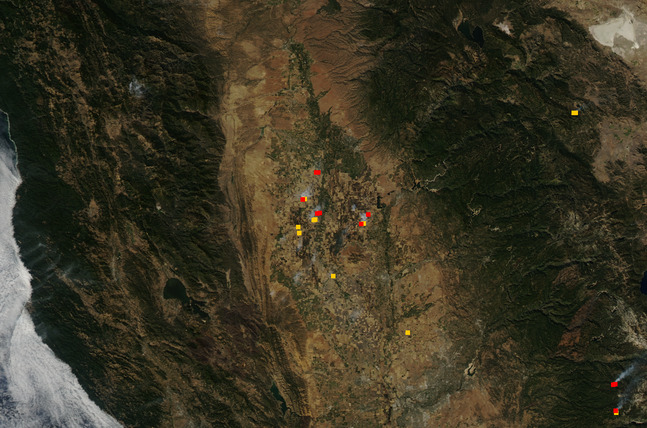
\includegraphics[width=\textwidth]{diagrams/injection/original.jpg}
        \caption{Original image with some fires.\newline}
        \label{fig:injection-orig}
    \end{subfigure}
    \begin{subfigure}{0.49\textwidth}
        \centering
        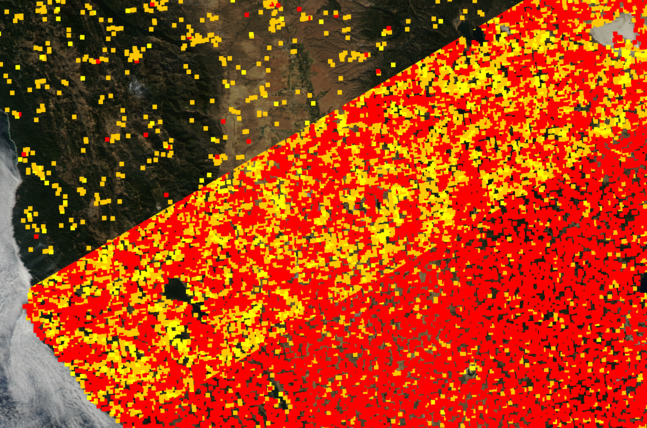
\includegraphics[width=\textwidth]{diagrams/injection/random_combined_diagonal.jpg}
        \caption{Fires randomly injected uniformly across the map. Composite of 3 images, with intensity of the fires increasing from top to bottom.}
        \label{fig:injection-random}
    \end{subfigure}
    \caption{An overview of the possible ways an attacker can manipulate the output of the forest fire detection algorithm by overshadowing the downlinked data. In each image, forest fires detected by the algorithm are highlighted in yellow, orange, and red in increasing order of intensity.}
    \label{fig:injection}
\end{figure*}

\begin{figure}
    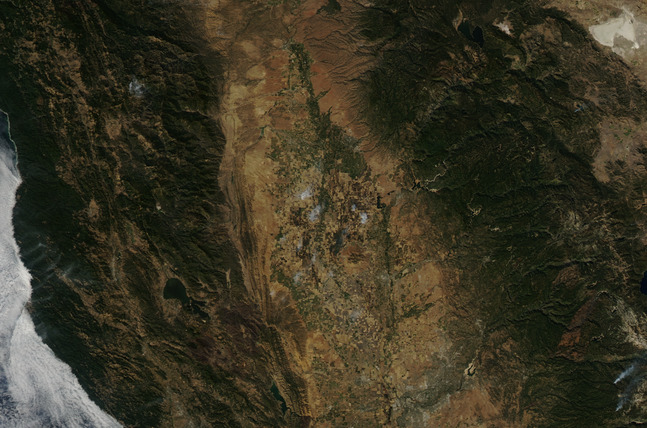
\includegraphics[width=\columnwidth]{diagrams/injection/masked_0.jpg}
    \caption{MODIS image with legitimate fires masked out.}
    \label{fig:injection-masked}
\end{figure}

In order to attack systems which rely upon Earth observing satellite data, the attacker must synthesise a malicious signal which decodes to the desired raw data.
When processed, this raw data will either poison the targeted satellite-derived dataset, or exploit a stage in the processing pipeline itself.
Then the attacker must overshadow a genuine broadcast with sufficient amplitude such that the targeted receiver decodes the attacker's signal.

In this section, we demonstrate the feasibility of each of these objectives with respect to a case study on FIRMS, NASA's forest fire detection system.
We firstly show in Section~\ref{sec:effects-on-processing-systems} how an attacker can generate an attack sequence which results in the injection of ficticious forest fires, the masking of existing ones, or the exploitation of vulnerabilities in the protocol decoding stages.
Since existing implementations of the EOS protocols are intended for decoding only, we firstly implement libraries to reencode the data.
We build upon these to demonstrate our attacks end-to-end on the FIRMS software, resulting in color-corrected images overlaid with the detected forest fires.

We go on to demonstrate the feasibility of the attack using only commercially available equipment through a series of radio overshadowing simulations.
The results demonstrate that a ground-based attacker can achieve the required overshadowing of a highly directional dish, for the budget of a motivated hobbyist.

\subsection{Effects on downlink processing systems}\label{sec:effects-on-processing-systems}

\subsubsection{Case Study: Injecting ficticious forest fires}

% If more time: describe the engineering re packet splitting across boundaries etc.

To successfully inject forest fires, an attacker needs to manipulate the infrared channels of MODIS packets within the downlinked data.
This data can either be obtained from distributed digital archive centers~\cite{ladsweb} beforehand, or in real time with access to a satellite dish.
In this example, the attacker is injecting forest firest at specific geographic coordinates, and so obtains data representing the desired target beforehand.
However, since all the information required to generate the data is present either from the known orbital parameters or within the data stream itself, forest fires could be similarly injected in real time.

% If more time: explain how the correct data is found wrt certain coordinates, in the long list
Data is available for download in the \textit{Level 0} format, which consists of MODIS SPP packets already decoded from the CADUs.
The archive lists packet data broken into short sequences according to the time at which the data was captured.
The attacker selects a sequence of packets corresponding to their targeted area, using the predictable orbital characteristics of the satellite to calculate the overpass time.

Once received, the attacker needs to modify the infrared sensor channels to draw fires at the desired locations.
By running the packet sequence through \textit{MODISL1DB\_SPA}, the attacker obtains the precise geographical coordinates of the boundaries of the image.
The attacker can target specific pixels in the image, since the sequence of packets encodes a scan over the image in a predicable pattern.
Specifically, the image is laid out as horizontal scan lines across the frame.
The number of the scan line is indicated in the secondary header, with the \textit{frame data count} increasing linearly throughout the scan.

Using this method, the attacker can determine the precise packets which, when modified will lead to the addition of forest fires at the desired coordiates.
However, since MOD14\_SPA detects fires through local peaks~\cite{mod14Manual}, the attacker can't write uniform values across large sequences of packets.
Forest fires are detected if instead the values within the desired area are set according to a random distribution.

Additionally, in order to have the image decode correctly, the attacker must be careful not to modify any non-sensor packets within the sequence.
For example, engineering packets are interspersed regularly throughout the sequence, which contain crucial timing information later used in the alignment of the scan lines between sensors.
Engineering packets are distinguished uniquely with a frame data count of zero, so an exception must be made to leave such packets unmodified.
Figure ~\ref{fig:interleave} demonstrates the partial result of an image with this timing data overwritten.

Finally, the attacker must reencode the SPP packet sequence into the CADU structure, aligning the packets within the structure accordind to the specification, recalculating the checksums, and applying the Viterbi encoding.
Figures~\ref{fig:injection} and~\ref{fig:location-injection} show the results of the FIRMS software stack within IPOPP decoding the resulting signal.


%Show the pipeline which results in the injection of ficticious fires, and the results
%Get a bit of info from Josh about how his pixel alignment works

\subsubsection{Case Study: Masking existing forest fires}

The attacker can also seek to mislead the fire detection algorithm through masking existing forest fires.
Unlike the case of creating ficticious fires, the attacker doesn't need to perform geolocation of the image, greatly simplifying the operation of processing the packets.
As a result, it becomes significantly easier to perform the attack in real time.

Data in this case study is instead obtained directly from an attacker receiver.
The bit sequence from the decoder must firstly be byte aligned and divided into CADUs, derandomised through Viterbi decoding depending on the satellite mode, and then error corrected according to the CADU checksum.
The result is an SPP MODIS packet sequence of equivalent form to those obtainable from the online archives.

The attacker can process the packet sequence with low latency, since the operation to each sensor packet is identical.
Specifically, the attacker needs to all of the infrared channels to a roughly uniform value.
Therefore, MOD14\_SPA fails to detect the requisite peaks, and the resulting dataset contains no marked fires.
The results can be seen in Figure~\ref{fig:injection-masked}.
